\documentclass[../main.tex]{subfiles}

\begin{document}
	\subsection{$I_{DS}$ function of $V_{GS}$}
	{
		
		\begin{tcolorbox}[colback=gray!5!white,colframe=gray!75!black]
			Plot, for the two types of transistors, the graph $I_{DS}(V_{DS}, V_{GS})$ for $V_{DS} \text{ constant } = V_{DD}$, and for $V_{GS}$ varying between between $V_{SS}$ and $V_{DD}$. Define graphically the threshold voltages $V_{tn}$ and $V_{tp}$ of the two types of transistors.
		\end{tcolorbox}
		
		\subsubsection{NMOS transistor}
		{
			
		We observe that $V_{DS} = V_{DD} \implies V_{DS} \geq V_{GS} - V_{tn} \implies$ the NMOS transistor is either cutoff or in saturation depending on the value of $V_{GS}$, thus
		
		\begin{equation}
			I_{DS}(V_{DS} = V_{DD}, V_{GS}) = 
			\begin{cases} 
				0, & \text{if } V_{GS} < V_{tn} \text{ (cutoff)}, \\[5pt]
				\frac{1}{2} k_n \frac{W}{L} (V_{GS} - V_{tn})^2, & \text{if } V_{GS} \geq V_{tn} \text{ (saturation)}.
			\end{cases}
		\end{equation}
		
		\begin{lstlisting}
			.include cmosws.mod
			
			Vds 2 0 dc 3.3V
			Vgs 1 0 dc 1V
			M1  2 1 0 0 MODN L=0.6U W=3.0U
			
			.dc Vgs 0 3.3 50mV
			.end
		\end{lstlisting}
		
		\begin{figure}[H]
			\centering
			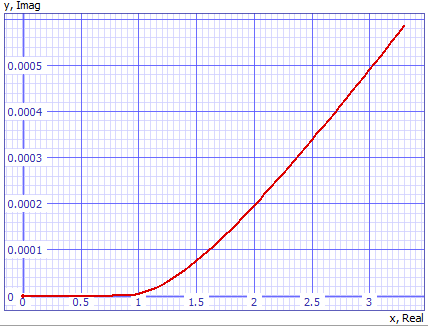
\includegraphics[width=0.5\textwidth]{plots/Q1_nmos.png}
			\caption{$I_{DS}$ function of $V_{GS}$ for NMOS transistor}
		\end{figure}
		
		We can define $V_{tn}$ graphically as the limit value where $I_{DS}$ becomes greater than $0$. We get $$V_{tn} \approx 0,87$$
		
		\begin{figure}[H]
			\centering
			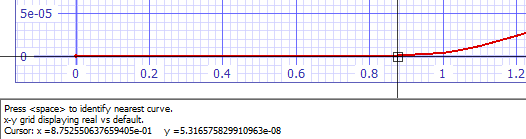
\includegraphics[width=0.5\textwidth]{plots/Q1_vtn.png}
			\caption{Determining $V_{tn}$}
		\end{figure}
		
		
		}
		\subsubsection{PMOS transistor}
		{
			
		In the PMOS transistor, to account for the reversed polarity we impose $V_{SD} = V_{DD} \implies V_{SD} \geq V_{SG} - V_{tp} $ where $V_{tp}$ is negative.
		
		Now, we expect
		
		\begin{equation}
			I_{DS}(V_{SD} = V_{DD}, V_{SG}) = 
			\begin{cases} 
				0, & \text{if } V_{SG} < |V_{tp}| \text{ (cutoff)}, \\[5pt]
				-\frac{1}{2} k_p \frac{W}{L} (V_{SG} - |V_{tp}|)^2, & \text{if } V_{SG} \geq |V_{tp}| \text{ (saturation)}.
			\end{cases}
		\end{equation}
		
		\begin{lstlisting}
			.include cmosws.mod
			
			Vsd 2 0 dc 3.3V
			Vsg 2 1 dc 1V
			M1  0 1 2 2 MODP L=0.6U W=6.0U
			
			.dc Vsg 0 3.3 50mV
			.end
		\end{lstlisting}
		
		Now, we can observe a curve equivalent to that of the NMOS transistor.
		
		\begin{figure}[H]
			\centering
			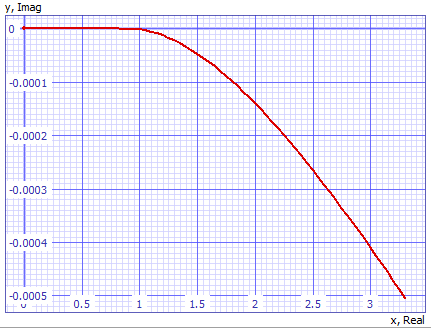
\includegraphics[width=0.5\textwidth]{plots/Q1_pmos.png}
			\caption{$I_{DS}$ function of $V_{SG}$ for PMOS transistor}
		\end{figure}
		
		We can identify $|V_{tp}|$ graphically as the limit value where $I_{DS}$ becomes smaller than $0$. We get $$V_{tp} \approx -0,82$$
		
		}
	}
\end{document}